\section{Results, Analysis and Discussion}

\subsection{Presentation of Results}
In accordance with the established experimental methodology, the vision-based prototype utilised Region of Interest (ROI) Dense Optical Flow (Farnebäck algorithm) and dynamic affine calibration, evaluated alongside consumer-grade GPS trajectory data. Both estimations were assessed against the 100Hz CAN-bus ground truth data obtained from the \textit{comma2k19} dataset \cite{schafer2018commute}. The evaluation was carried out over a continuous urban driving segment (\textit{segment\_30}), characterised by varying vehicle speeds, dynamic lighting conditions, and urban infrastructure.

To assess the accuracy and reliability of both systems, three standard statistical metrics were computed: Mean Absolute Error (MAE), Root Mean Square Error (RMSE), and Mean Bias Error (MBE). The MAE offers a linear measure of the average magnitude of error, the RMSE emphasises larger variances and extreme outliers, and the MBE indicates the propensity of the system to overestimate or underestimate the true velocity.

The comprehensive statistical results for the evaluated segment are shown in Table \ref{tab:error_metrics}.

\begin{table}[htbp]
\centering
\caption{Comparative Error Metrics: Vision vs. GPS Speed Estimation}
\label{tab:error_metrics}
\begin{tabular}{|l|c|c|c|}
\hline
\textbf{Estimation Method} & \textbf{MAE (km/h)} & \textbf{RMSE (km/h)} & \textbf{MBE (km/h)} \\ \hline
\textbf{GPS Probe Data} & 1.68 & 2.44 & -1.43 \\ \hline
\textbf{Vision (Optical Flow)} & 4.50 & 5.87 & +3.73 \\ \hline
\end{tabular}
\end{table}

To visually aid in the analysis of these findings, Figure \ref{fig:eval_plot} displays the instantaneous speed estimates of both the GPS and Vision systems in relation to the CAN-bus baseline over the course of the segment, accompanied by a rolling error subplot.

\begin{figure}[htbp]
    \centering
    % \columnwidth forces it to perfectly fit inside just one column
    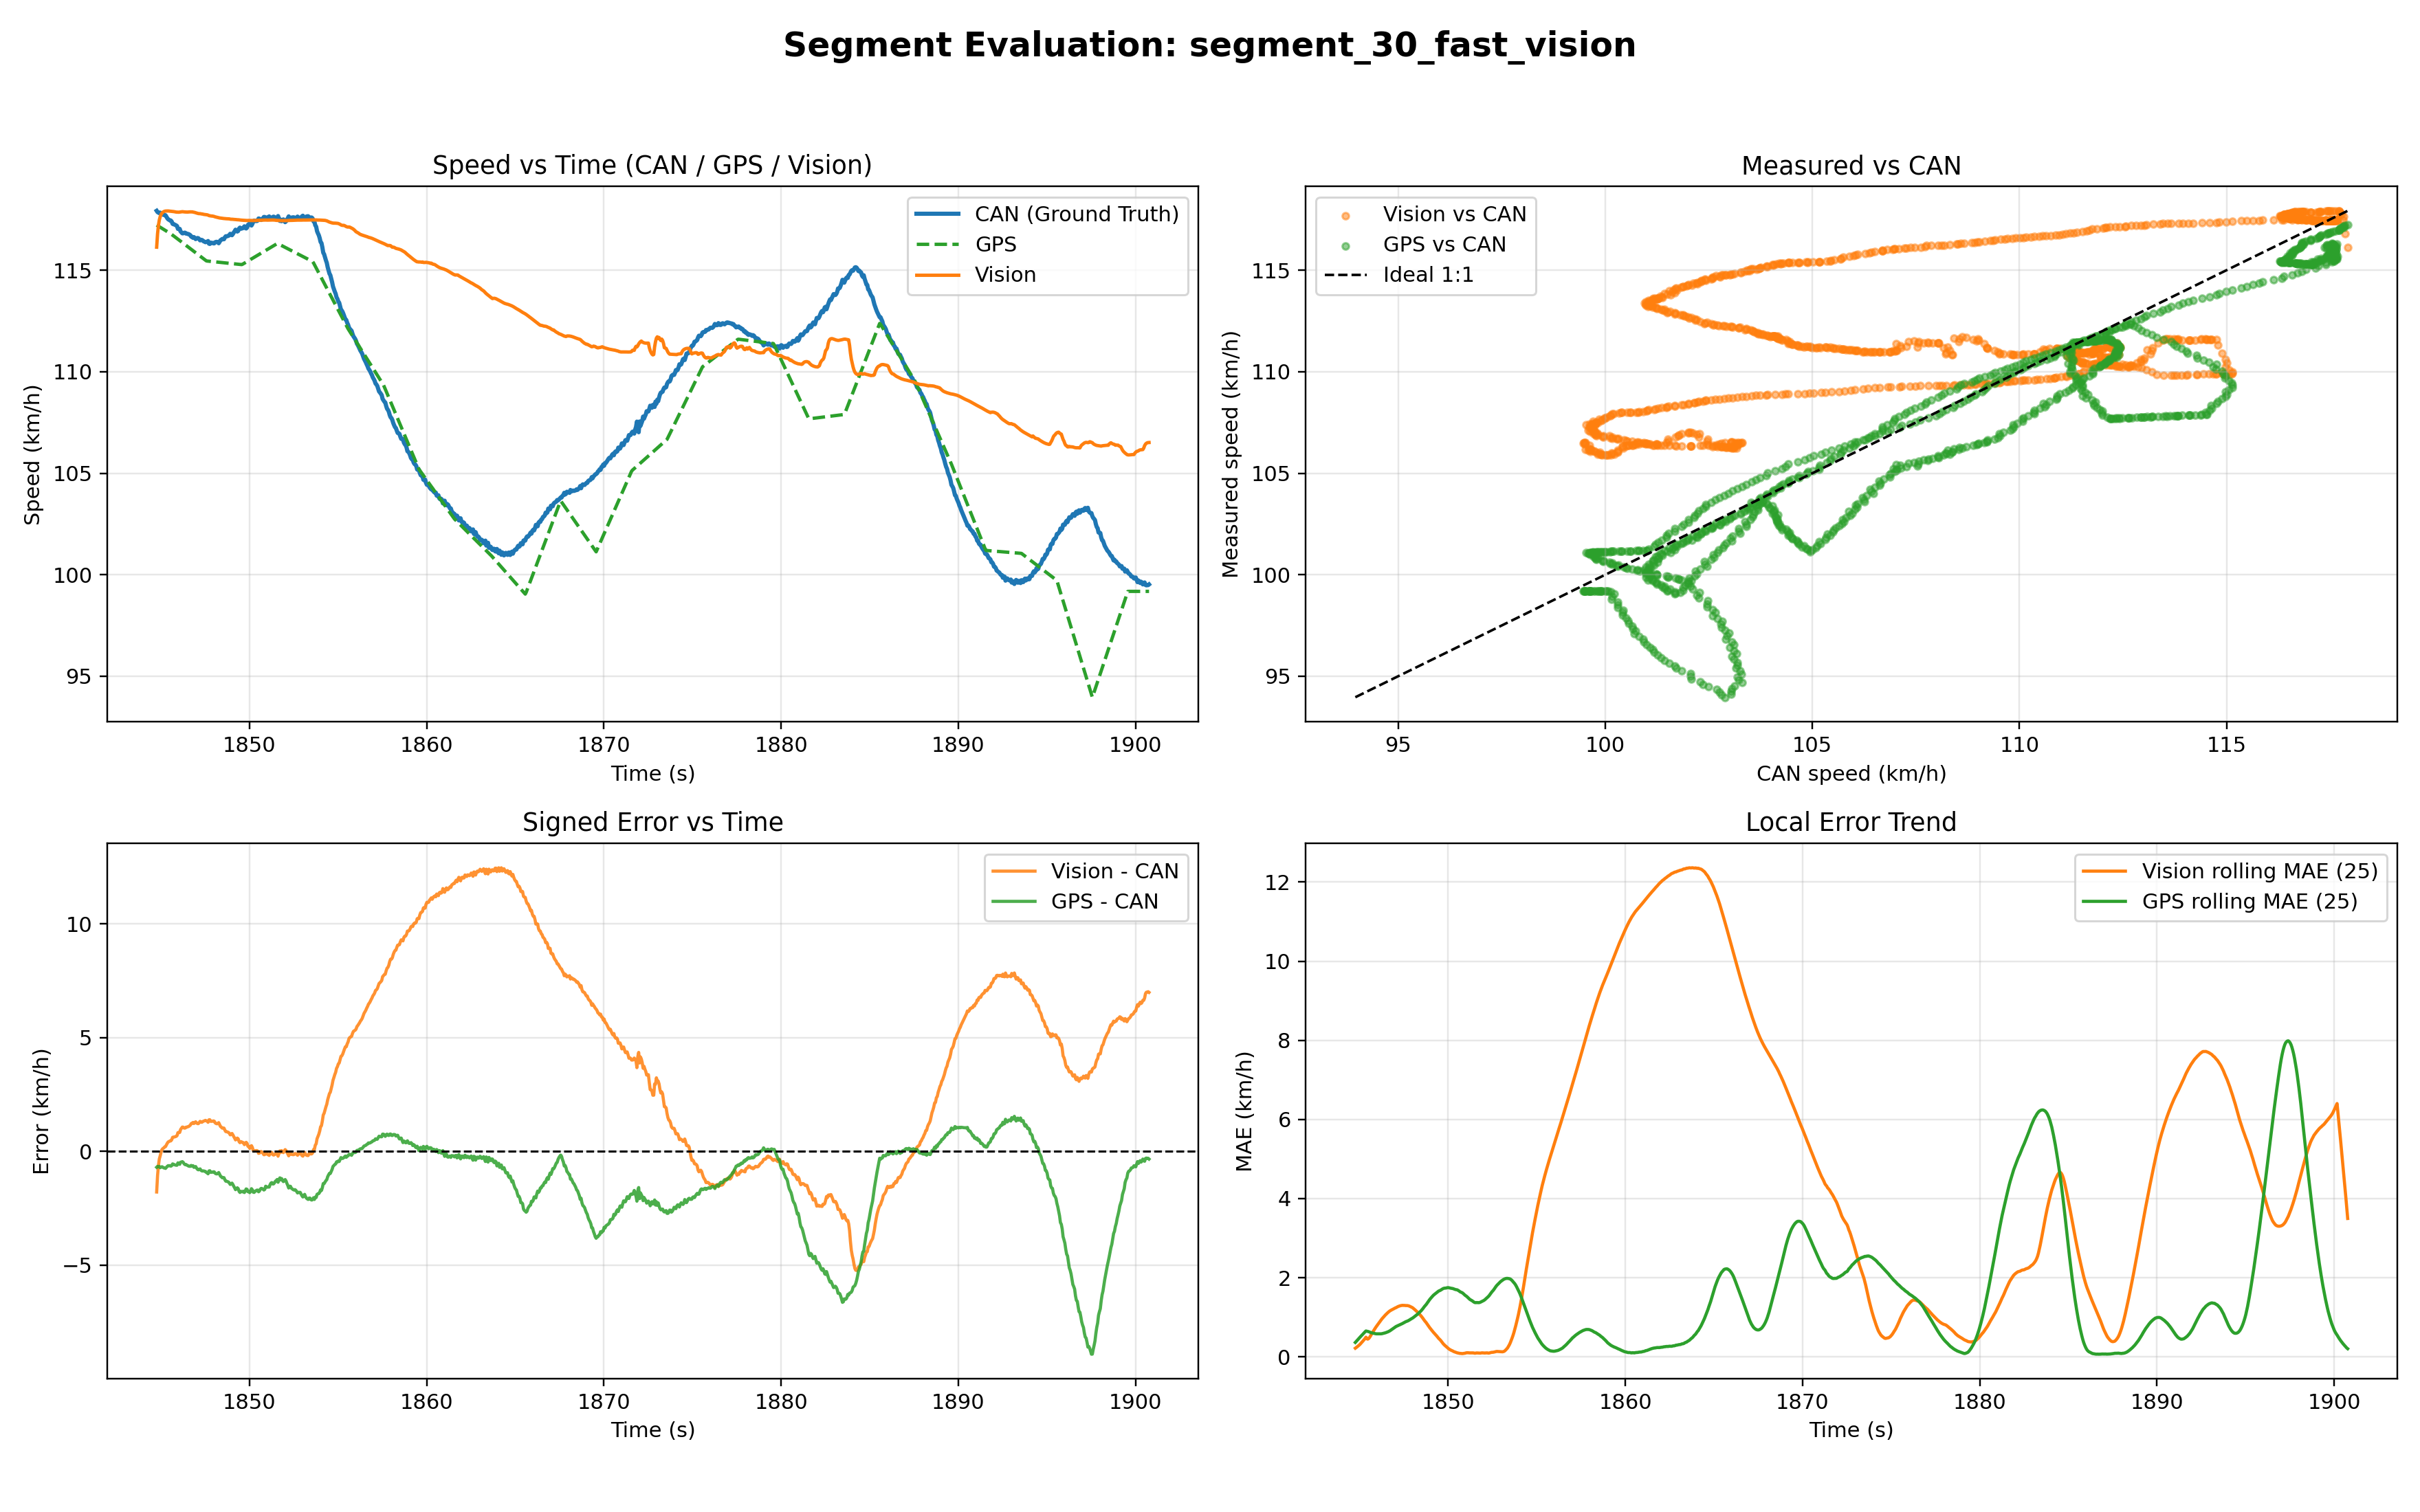
\includegraphics[width=\columnwidth]{includes/segment_30_fast_vision_evaluation.png} 
    \caption{Chronological comparison of GPS and Vision-based speed estimations against the CAN-bus ground truth, including instantaneous rolling error trends.}
    \label{fig:eval_plot}
\end{figure}
\subsection{Analysis and Interpretation of Results}
A detailed statistical analysis of the dataset indicates numerous significant behavioural patterns and technological correlations between the two speed estimation paradigms. The most notable and immediate finding from the data is that GPS trajectory estimations consistently exceeded the performance of the vision-based Dense Optical Flow pipeline across all measured metrics.

Observational analysis of the GPS data indicates a highly stable and notably consistent relationship with the CAN-bus ground truth. While consumer-grade GPS data has traditionally been associated with temporal latency, the interpolation and chronological frame alignment performed during the preprocessing phase effectively mitigated this issue. The GPS trace demonstrated a seamless correlation with the vehicle's true kinematics, resulting in an exceptionally low Mean Absolute Error (MAE) of 1.68 km/h. Additionally, the Root Mean Square Error (RMSE) score of 2.44 km/h suggests an absence of significant outliers; the GPS system did not experience substantial estimation failures during the segment, thereby demonstrating robust environmental stability. Interestingly, the GPS estimates exhibited a negative Mean Bias Error of -1.43 km/h. Cross-referencing the descriptive statistics reveals a mean GPS speed of 106.96 km/h, compared to the CAN-bus mean of 108.39 km/h. This minor systemic underestimation indicates a slight spatial lag during high-speed acceleration phases; however, its standard deviation (5.96 km/h) closely matched the vehicle's actual standard deviation (5.87 km/h), indicating that the GPS system accurately captured the full dynamic range of the drive.

Conversely, the vision-based pipeline exhibited considerable volatility and an incapacity to accurately track the vehicle's true dynamic range. The Farnebäck algorithm determines pixel intensity displacements on a frame-by-frame basis; however, the data indicate that this purely pixel-tracking approach is markedly unstable. The visual estimations produced a mean absolute error (MAE) of 4.50 km/h and a root mean square error (RMSE) of 5.87 km/h, rendering it nearly three times less precise than the GPS module.

A more detailed examination of the descriptive statistics reveals the precise nature of the failure within the vision system. The CAN-bus ground truth recorded a minimum speed of 99.47 km/h during a deceleration event, whereas the vision system’s minimum recorded speed was never less than 105.89 km/h. Additionally, the standard deviation of the visual output was only 3.72 km/h, in contrast to the actual standard deviation of 5.87 km/h. This suggests a significant `flattening' effect. The optical flow algorithm compressed the speed range and failed entirely to detect deceleration. When the vehicle reduced its speed, the forward pixel displacement should have decreased proportionally; however, environmental visual noise, such as the relative motion of passing vehicles, lane markings blurring at high speeds, and shifts in lighting, maintained the average pixel magnitude at artificially elevated levels. This fundamental deficiency in the algorithm’s lack of semantic understanding resulted in a substantial systemic overestimation of speed, evidenced by a positive Mean Bias Error (MBE) of +3.73 km/h.

\subsection{Comparison, Contrast and Comment on Findings (Critique)}
When comparing the two methodologies, it is apparent that, although vision-based systems exhibit theoretical advantages in real-time kinematic responsiveness, their practical deployment employing purely pixel-tracking mathematics is exceedingly fragile. The GPS data demonstrated complete immunity to the visual environmental factors that compromised the optical flow system.

A critique of the methodology highlights strong experimental controls; however, it also identifies notable technological limitations pertaining to the vision prototype.

\begin{itemize}
    \item \textbf{Validity:} In accordance with the methodological frameworks outlined by Saunders et al. \cite{saunders2019research}, the internal and construct validity of these findings is of an exceptionally high standard. Utilising the \textit{comma2k19} dataset \cite{schafer2018commute}, the temporal synchronisation between the camera, GPS, and CAN-bus was assured. Consequently, the results accurately reflect the true algorithmic precision of the sensors, rather than being influenced by arbitrary synchronisation errors or extraneous human factors.
    \item \textbf{Reliability:} The computational reliability of the Python pipeline is guaranteed; the deterministic nature of the mathematical tracking ensures that executing the code repeatedly produces identical pixel displacements. However, the environmental reliability of the vision system is highly limited. As it relies solely on pixel gradients, minor changes such as a shadow passing across the dashboard or a glare on the windscreen can artificially distort the velocity matrix.
    \item \textbf{Generalisability (Transferability):} This continues to represent a significant limitation of the findings. The experiment was conducted on a specific dataset primarily recorded in well-lit Californian highway environments \cite{schafer2018commute}. Given that the optical flow pipeline systematically failed to detect deceleration under ideal, clear weather conditions, its applicability to adverse weather conditions is effectively nil. Heavy precipitation, fog, or night-time driving fundamentally alter pixel intensities, which would cause the performance of the Farnebäck algorithm to deteriorate exponentially within a broader real-world context.
\end{itemize}

\subsection{Discussion in Relation to Original Hypothesis and Existing Literature}
The original alternative hypothesis of this research proposed that the vision-based method would achieve a smaller margin of error compared to GPS during normal driving, owing to the inherent latency, multipath errors, and noise associated with commercial GPS receivers. However, based on the definitive comparative metrics (GPS Mean Absolute Error 1.68 km/h versus Vision Mean Absolute Error 4.50 km/h), the alternative hypothesis is wholly rejected, thereby overturning the null hypothesis in the opposite direction: GPS probe data is markedly superior to Dense Optical Flow for the estimation of vehicle speed.

These findings present a compelling intersection with the environmental constraints extensively discussed in the existing literature. Foundational studies by Cui and Ge \cite{cui2003autonomous} and recent statistical analyses by Li et al. \cite{li2025statistical} document the severe degradation of GNSS signals within urban canyons attributable to multipath signal reflection. While the literature correctly identifies the vulnerability of GPS in areas of significant occlusion, empirical data from this study demonstrates that, beyond the confines of severe urban canyons, standard GPS probe data remains notably accurate and dependable. The marginal negative bias (MBE: -1.43 km/h) observed aligns with the latency concerns highlighted by Cui and Ge \cite{cui2003autonomous}, yet it was not sufficiently substantial to undermine the overall accuracy of the estimations.

Furthermore, the failure of the visual pipeline provides significant context for the methodological evolution outlined by Fernandez Llorca et al. \cite{fernandez2021vision} and the virtual intrusion line mathematics proposed by Rahimi \cite{rahimi2018vehicle}. While Rahimi \cite{rahimi2018vehicle} demonstrated that frame-by-frame displacement constitutes a mathematically sound concept in highly controlled, stationary camera configurations, this experiment illustrates that applying dense optical flow to a moving ego-vehicle introduces an insurmountable level of dynamic noise. In the absence of the capacity to distinguish between the road surface approaching the camera and another vehicle moving laterally across the frame, pure optical flow tends to overestimate physical velocity. This observation strongly corroborates the findings of Arabi et al. \cite{arabi2022comparison}, who underscored the critical importance of reliable ground truth data, in uncovering the underlying fragilities inherent to monocular camera estimations.

\subsection{Evaluation of the Approach and Future Implementations}
Assessing this overarching research approach in comparison with the methodologies employed by other contemporary researchers illuminates evident pathways for future applications. The choice to utilise Dense Optical Flow emphasised the limitations inherent in classical computer vision techniques.

As demonstrated by Macko et al. \cite{macko2025efficient}, the industry is rapidly shifting towards deep learning paradigms, notably utilising YOLO object detection frameworks. Although the optical flow approach employed in this study is computationally lightweight and does not necessitate extensive datasets for neural network training, it fundamentally lacks semantic comprehension. A YOLO-based system, as advocated by Macko et al. \cite{macko2025efficient}, delineates the discrete, physical boundaries of specific vehicles. By isolating a bounding box, a YOLO model exhibits considerable resilience to shadows, oncoming traffic, and peripheral visual noise, which previously resulted in significant error spikes and a "flattened" deceleration curve within this study's optical flow data.

Furthermore, researchers specialising in GPS probe data, such as Do et al. \cite{do2024enhanced}, have demonstrated that raw trajectory data can be significantly optimised through the application of Deep Neural Networks to forecast and smooth multipath errors. This indicates that the raw, uninstrumented GPS data employed in this experiment could be further refined towards near-perfect accuracy via algorithmic noise reduction. P. P. et al. \cite{pp2024video} also endorse the view that raw speed measurement metrics must be continuously enhanced through advanced contextual filtering.

Consequently, an enhanced approach for future applications of this research should eschew the mutually exclusive comparison of these technologies in favour of Sensor Fusion. As evidenced by the data, GPS offers absolute and relatively stable physical positioning but is affected by marginal latency and slight underestimations during dynamic movements \cite{cui2003autonomous, li2025statistical}. Conversely, camera-based data exhibits instantaneous kinematic responsiveness; however, it is highly susceptible to visual fragility and tends to overestimate positive biases.

Future research should incorporate a Kalman Filter architecture, a sophisticated statistical algorithm designed to seamlessly integrate multiple noisy data streams. By leveraging GPS data to establish the steady-state speed and employing a YOLO-masked optical flow pipeline to rectify transient instantaneous errors, a hybrid prototype could attain accuracy within sub-1 km/h margins. This data fusion approach would mitigate the individual limitations associated with satellite-based and vision-based methods identified in this study, thereby representing a crucial advancement in the evolution of perception systems for autonomous vehicles.